% !TEX root = ./../main.tex
\chapter{Model of cell membrane and monolayer--protected NP}
\label{chap:membraneNP}
In the first part of this chapter we will present and describe the model of the charged monolayer--protected 
\ac{AuNP} developed by Federica Simonelli and co--workers in \cite{simonelliThesis} and \cite{ourPaper}. The gold 
core is treated by an all atoms representation, while the ligands are modeled at \ac{CG} level by the \martini 
\ac{FF}. In the second part of the chapter we will describe the most important physical and chemical features of 
the cell membrane. Then we will summarize the characteristics of the \ac{CG} model used to treat it. Finally, we 
will describe the interaction mechanism and some preliminary thermodynamic results about the interaction of the 
\ac{AuNP} and the model cell membrane, as outlined in \cite{ourPaper}. For a more precise discussion about the 
\ac{NP}--membrane interaction and the models parameterization the reader is addressed to the work of Federica 
Simonelli \etal\, \cite{ourPaper} and her thesis work \cite{simonelliThesis}. For more details about the gold core used, its properties, equilibrium structure and so forth, the reader is addressed to the work of Lopez-Acevedo \etal\, \cite{clusterEquilibrium} while for a general discussion about thiolated \acp{AuNP} to the work of Häkkinen \cite{corePassivated}. For what concerns cell membranes and biological lipids the reader is addressed to the book of Yeagle \cite{yeagle}.

\section{NanoParticle model}
% gold core --> Thyiol passivated --> ligands
%Ligand Composition: Patched (1:1), Random (1:1) (1:2)
%Different level of hydrophobicity
%Different ligand charge: anionic/cationic NP
Monolayer--protected \acp{AuNP} have the advantage of having a well defined molecular structure. That is, 
mono--dispersed solutions can be synthesized and structurally determined. In particular \acp{AuNP} are 
biocompatible, have a facile surface chemistry and efficiently convert light into heat. Monolayer--protected 
\acp{AuNP} have a definite mass and molecular composition, and their structure is stabilized by the covalently 
bound ligands shell. Most commonly they are thiolated compounds because they covalently bound to the gold \ac{NP} 
by Au--S surface bonds, that is, a robust but modifiable interaction, crucial in stabilizing the \ac{NP} and 
transmitting electronic interactions between gold and sulfur--containing organic molecules \cite{corePassivated}. 
Moreover monodisperse \acp{AuNP} can be synthesized in the $1-4$~nm range. Subtle changes of size, structure and 
ligand compositions and arrangements, can affect \ac{NP} properties such as their optical properties, important 
for biological sensing and therapeutics. 
%Thiolated \acp{AuNP} are air stable, electrochemically stable and thermally stable compounds [].
Several stable thiolated \acp{AuNP} are identified, differing in size of the gold core and number of ligands 
\cite{corePassivated}. In this thesis work we will consider the {Au$_{144}$(SR)$_{60}$} thiolated \ac{AuNP}, where 
R are the aliphatic chain of the thiol compounds. The equilibrium structure of the gold core is described by 
\textit{ab--initio} calculation in \cite{clusterEquilibrium}. 

Changing the composition of the aliphatic chains bonded to the thiol group, different properties of the thiolated 
\ac{AuNP} can be achieved, such as different net charge, different level of hydrophobicity, different size and so 
on. In particular, as we shall see, in the model we will use we consider only \ac{OT} and \ac{MUS} ligands that 
cover the \ac{NP} gold core with a monolayer with different compositions and surface arrangements. 
%To overcome the computational cost of an atomistic model we use a \martini \ac{CG} model of the \ac{OT} and \ac{MUS} ligands. 

%The model of the \ac{AuNP} and the \martini model of the \ac{OT} and \ac{MUS} ligands are developed by Federica Simonelli \etal\, in \cite{ourPaper}, and the reader is addressed to it for a more detail discussion about the model and the parameterization.

\subsection{Passivated gold core}
% some information about gold core: dimensions, number of atoms, model used, elastic network, shel construction
The gold core is composed of $144$ atoms, it has icosahedral symmetry and it is made of three bulk shell with 
$12$, $42$ and $60$ atoms, respectively. A surface shell of $30$ atoms completes the gold cluster structure. Then 
$60$ sulphur atoms, which bind the aliphatic chains (R) to the gold core, are bounded to the gold atoms on the 
surface through the typical bond structure RS--Au--SR. The shell construction is shown in 
figure~(\ref{fig:goldShell}).
\begin{figure}[!ht]
	\centering
	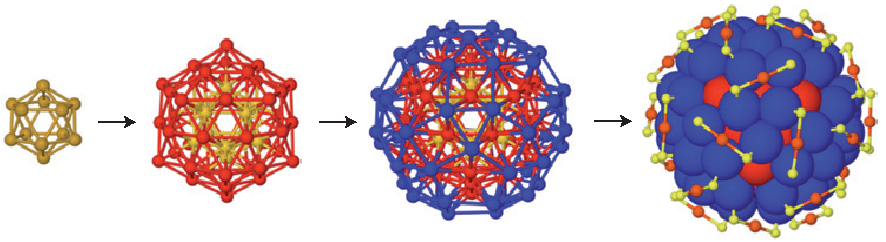
\includegraphics[width=0.8\textwidth]{./img/goldShell}
	\caption{First three frame: the concentric $12$--(yellow), $42$--(red) and $60$--(blue) atom gold internal shell, surrounded (last frame) by $30$ gold (red small) and $60$ sulphur (yellow small) surface atoms. The R chains are not shown. Taken from \cite{corePassivated}.}
	\label{fig:goldShell}
\end{figure}

The resulting diameter of the gold core is about $2$~nm. When passivated by thiols, its overall size depends on 
the length of the aliphatic chains bound to the sulphur atoms. The monolayer--protected \acp{AuNP} we will 
consider have a total diameter of about $4$~nm.

Despite the computational cost associated to atomistically describe the \ac{NP} core, all gold and sulfur atoms 
are taken into account. Bonds between gold atoms and sulfur atoms are allowed to vibrate. As we have seen in a 
previous section, a many--body potential should be used. Instead, as we are interested in the vibrational modes of the core atoms, 
%Federica Simonelli in her thesis work, found that
a more efficient way, as shown in figure~(\ref{fig:coreNetwork}), is to use an elastic network associate the 
potential energy
\begin{equation*}
	U = \frac{1}{2}\sum_i \sideset{}{'}\sum_{j\ne i}k_{ij}(r_{ij} - r_{ij}^0)^2
\end{equation*}
where $r_{ij}$ is the distance, $k_{ij}$ is the bond constant for $i-j$ atom pair and the prime indicates that 
only neighbor atoms within a certain cutoff are considered. 
\begin{figure}[h!t]
	\centering%
	\subfloat[Gold elastic network]{%
		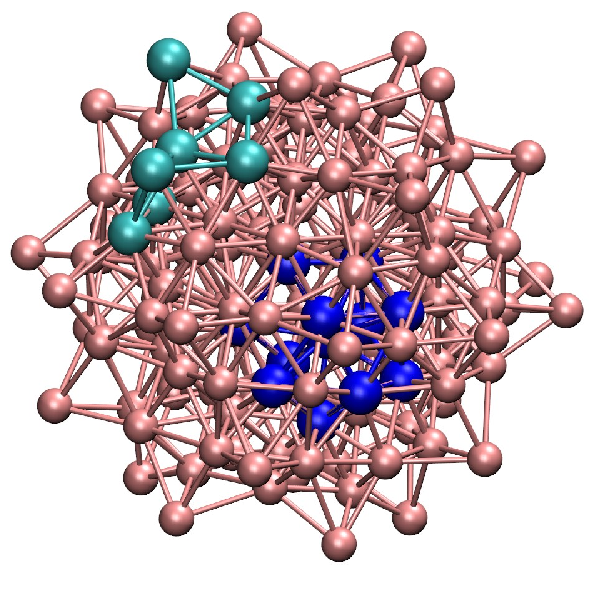
\includegraphics[width=0.35\textwidth]{./img/goldNetwork}%
	}\qquad%
	\subfloat[\acs{AuNP} cluter]{%
		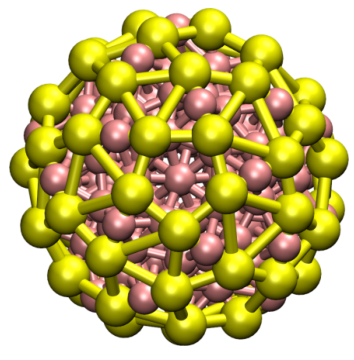
\includegraphics[width=0.32\textwidth]{./img/NPCluster}%
	}
	\caption{Left: gold elastic network. In cyan a surface atom and its neighbors; in blue bulk atom and its neighbors. Right: \acs{AuNP} cluster. The elastic network for both gold and sulfur atoms are represented by sticks. Taken from \cite{simonelliThesis} and \cite{ourPaper}.}
	\label{fig:coreNetwork}
\end{figure}

%The bond constants is assigned so as to reproduce the vibrational spectrum of the gold core as provided by the many--body Gupta potential. 
The bond constant is assigned to $k = 32500$~kJ/(mol\,nm$^2$) for Au--Au surface atoms, $k = 11000$ kJ/(mol\ 
nm$^2$) for Au--Au bulk atoms, $k = 1250$~kJ/(mol\,nm$^2$) for S--S atoms and $k = 32500$~kJ/(mol\,nm$^2$) for 
Au--S bonds, as summarized in table~(\ref{tab:NPConstants}). Instead, the equilibrium distances are derived from 
\textit{ab--initio} data in \cite{clusterEquilibrium}. Moreover, to prevent the penetration of other particles 
inside the \ac{NP} core, a purely repulsive interaction of the form $C/r^{-12}$ where 
$C = 0.92953\cdot 10^{-6}$~(kJ\,nm$^{12}$)/mol, is added between gold and sulfur atoms, gold and all other 
particles and sulfur and all other particles. A gold atom is considered as bulk atom if it has at least nine gold 
atom neighbors otherwise as a surface atom. Two gold atoms $i$ and $j$ are neighbors if their distance is 
$r_{ij} \le 0.35$~nm. Instead, two sulfur atoms are considered neighbors if they lie in a sphere shell of radius 
$0.55$~nm, i.e. each sulfur atom have at least five neighbors.
\begin{table}[h!t]
	\centering
	\begin{tabular}{lr}
		\toprule
		Bond			 & $k$\,\footnotesize[kJ/(mol\,nm$^2$)] \\ \toprule
		Au--Au (bulk) 	 & $11000$ 	\\ \midrule
		Au--Au (surface) & $32500$ 	\\ \midrule
		Au--S			 & $32500$ 	\\ \midrule
		S--S			 & $1250$ 	\\ \bottomrule
	\end{tabular}
	\caption{Summary of the bond constants for the elastic network of the \acs{NP} core.}
	\label{tab:NPConstants}
\end{table}

\subsection{Functionalizing ligands}
Our \ac{AuNP} core is functionalized with \ac{MUS} and \ac{OT} ligands as shown in figure~\ref{fig:figands}. 
\ac{MUS} is a charged compound made of an alkyl chain (\acs{CH2})$_{11}$ and a charged terminal \acs{SO4-} group. 
The charged terminal group makes \ac{MUS} partially hydrophilic. \ac{OT}, instead, is completely hydrophobic and 
it is made by an alkyl chain (\acs{CH2})$_{7}$ and one \acs{CH3} terminal group. Using both hydrophilic and 
hydrophobic groups guarantees that \acp{NP} are stable, that is, they do not aggregate in aqueous environments.
\begin{figure}[!ht]
	\centering
	\subfloat[\acs{OT} ligand]{%
		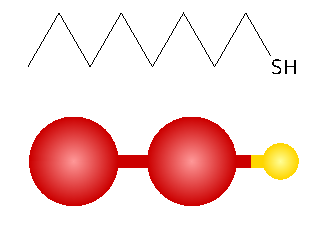
\includegraphics[width=0.3\textwidth]{./img/OT/OT}%
		\label{fig:ot}%
	}%
	\qquad\qquad%
	\subfloat[\acs{MUS} ligand]{%
		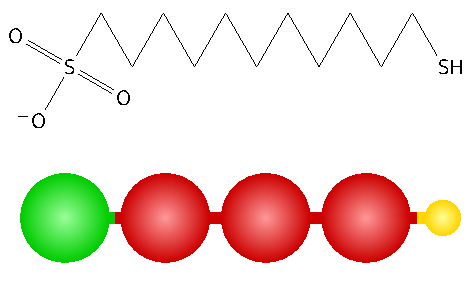
\includegraphics[width=0.35\textwidth]{./img/MUS/MUS}%
		\label{fig:mus}%
	}%
	\caption{Top: chemical structure. Bottom: \acs{CG} \martini model (red: C$_1$ bead, green: Qda negatively charged bead and yellow: sulfur atom).}
	\label{fig:figands}
\end{figure}

\paragraph{\textbf{OT Model}} Two \martini beads of type C$_1$ model the eight carbon atoms of the \ac{OT} 
backbone and their hydrogen atoms. The chemical structure and the resulting \ac{CG} \martini model is shown in 
figure~(\ref{fig:ot}). The first bead of each \ac{OT} ligand is bound to a sulphur atom via a harmonic potential 
with a bond constant of $1250$~kJ/(mol\,nm$^2$) and equilibrium length of $0.47$~nm. The second bead is connected 
to the first by the same bond potential. An angle potential as in equation~\eqref{eq:martiniAngle} is used among 
the three particles. Parameters are fixed in accordance with the standard \martini parameters for alkanes. 
%Moreover a purely repulsive potential, as described previously, is used between C$_1$ beads and gold and sulfur 
%atoms to prevent the penetration of the \ac{NP} core.

\paragraph{\textbf{MUS Model}} Three \martini beads of type C$_1$ model the hydrophobic chain of the \ac{MUS} 
ligand. The charged group is modeled as a Qda bead with a charge of $-\mathsf{e}$. The chemical structure and the 
resulting \ac{CG} \martini model is shown in figure~(\ref{fig:mus}). Even in this case the first bead of a 
\ac{MUS} ligand is bound to the sulphur atom through a harmonic potential with the same parameter: bond constant 
of $1250$~kJ/(mol\,nm$^2$) and equilibrium length of $0.47$~nm. The same potential is used to bind all other 
beads to the previous one. An angle potential as in equation~\eqref{eq:martiniAngle} is used among the sulfur 
atom, the first C$_1$ and second C$_1$, among the first, the second and the third C$_1$ beads and so on for all 
four beads. Parameters are fixed in accordance with the standard \martini parameters for alkanes.
%As in the \ac{OT} ligand 
%model, a purely repulsive potential, as described previously, is used between C$_1$ beads and gold and sulfur 
%atoms to prevent the \ac{NP} penetration. The same applies between Qda bead and gold and sulfur atoms.

\paragraph{\textbf{level of hydrophobicity}} The \ac{AuNP} core can be functionalized with both ligands at 
different composition. In particular varying the ratio between the \ac{OT} and \ac{MUS} ligands different levels 
of hydrophobicity can be reached. Two surface compositions will be considered in this thesis work: 
(\ac{MUS}:\ac{OT} $1$:$1$) and (2:1), the former is the main used in this thesis work. This choice is due to the 
possibility to compare to previous experimental and simulation data \cite{Maccarini2013}, \cite{VanLehn2013}, 
\cite{VanLehn2014} and \cite{VanLehn2015}.

\paragraph{\textbf{surface arrangements}} The ligands on the \ac{AuNP} surface can be arranged in two possible 
ways: randomly or with a predetermined scheme. We will consider both \acp{NP} with a random ligand arrangement 
and \acp{NP} with a striped ligand arrangement. The striped scheme is obtained dividing the \ac{NP} surface in 
three stripes: the external two stripes are covered with \ac{MUS} ligands while the central with \ac{OT} ligands. 
For this thesis work we consider three type of \acp{NP}: striped (\ac{MUS}:\ac{OT} $1$:$1$), random 
(\ac{MUS}:\ac{OT} $1$:$1$) and random (\ac{MUS}:\ac{OT} $2$:$1$). In figure~(\ref{fig:coating}) the different 
coatings for the \ac{NP} core is shown.

\begin{figure}[!ht]
	\centering
	\subfloat[striped ($1$:$1$)]{
		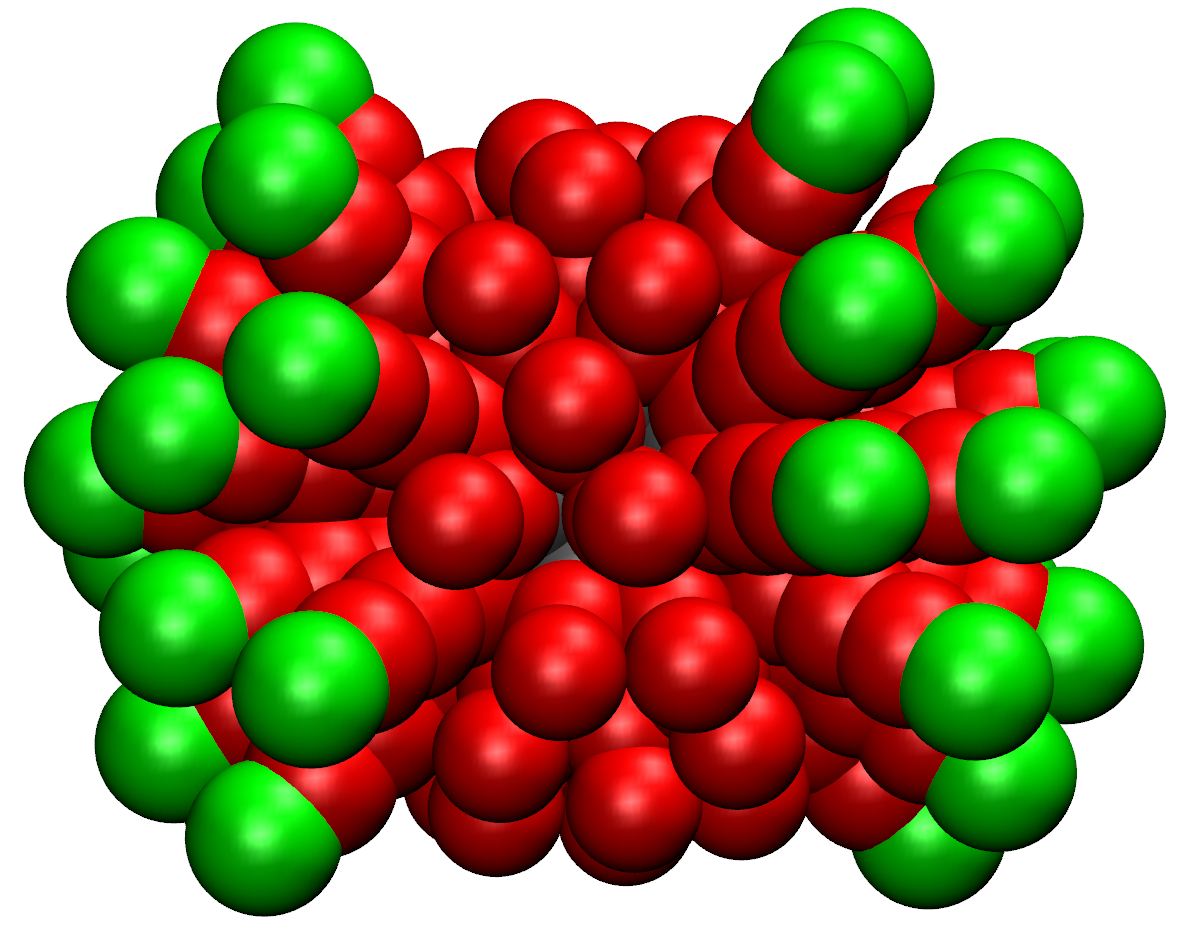
\includegraphics[width=3.3cm]{./img/coatings/striped}
	}%
	\qquad
	\subfloat[random ($1$:$1$)]{
		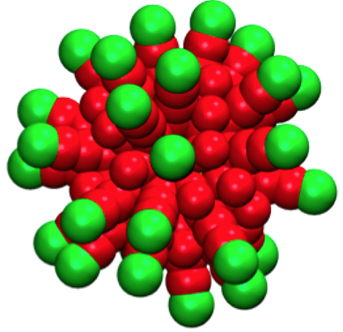
\includegraphics[width=2.9cm]{./img/coatings/random11}
	}%
	\qquad
	\subfloat[random ($2$:$1$)]{
		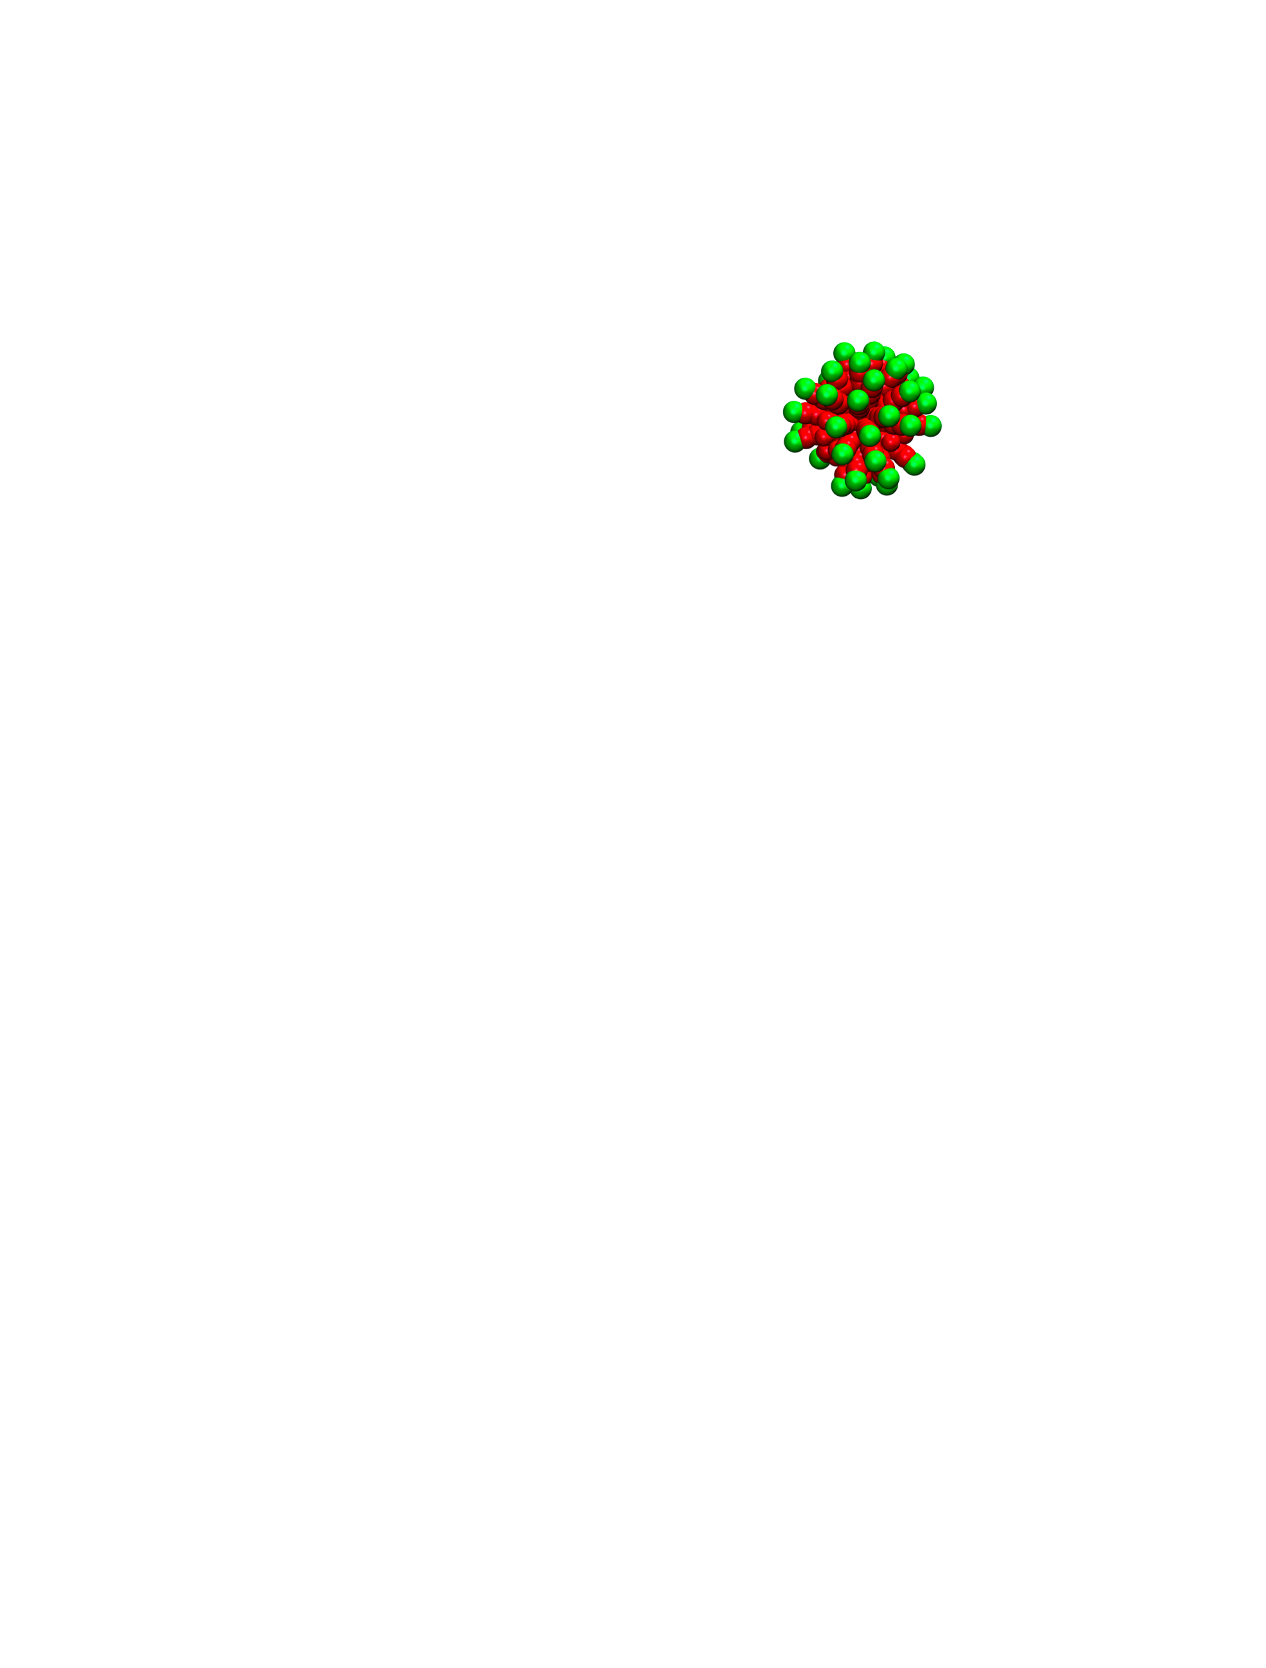
\includegraphics[width=2.7cm]{./img/coatings/random21}
	}%
	\caption{Au\acs{NP} with different ligands surface arrangements and composition. From left to right: striped (\ac{MUS}:\ac{OT} $1$:$1$), random (\ac{MUS}:\ac{OT} $1$:$1$) and random (\ac{MUS}:\ac{OT} $2$:$1$). Hydrophobic beads are shown in red while the negatively charged beads are green.}
	\label{fig:coating}
\end{figure}

\section{Cell membranes}
The cell membrane or cytoplasmic membrane is a biological membrane that separate the interior and the external environments of a living cells and controls communications and nutrient flow into and out the cell. This is essential to enable the function and stabilize the structure of cells. The membrane main function is the compartmentalization of a biological environment into two well defined not independent subsection: the cell in which the ``life reactions'' take place and the external cell fluid in which all the necessary biological compounds are dissolved. The compartmentalization in such environments enhance the probability of chemical reactions to take place but also allow to develop different chemical reactions inside and outside the cell. From an evolutionary point of view it is believed that a simple membrane that defines an inside and an outside environments and that protect and concentrates molecules in a closed space, it was necessary for the development of life. 

\subsection{Real cell membranes}
Since the compartmentalization, the cell membrane have to allow the exchange of biological molecules from and to the outside world. This role is, in a small part, fulfilled by the membrane itself through the passive translocation of small molecules or ions. But the main part is fulfilled through proteins and other compounds that are solved inside the membrane. As we can see from a cartoon of a real cell membrane in figure~(\ref{fig:cellMembrane}), the biological membrane is a crowded environment consisting of phospholipids, glycolipids, carbohydrates, proteins and other organic molecules.
\begin{figure}[!ht]
	\centering
	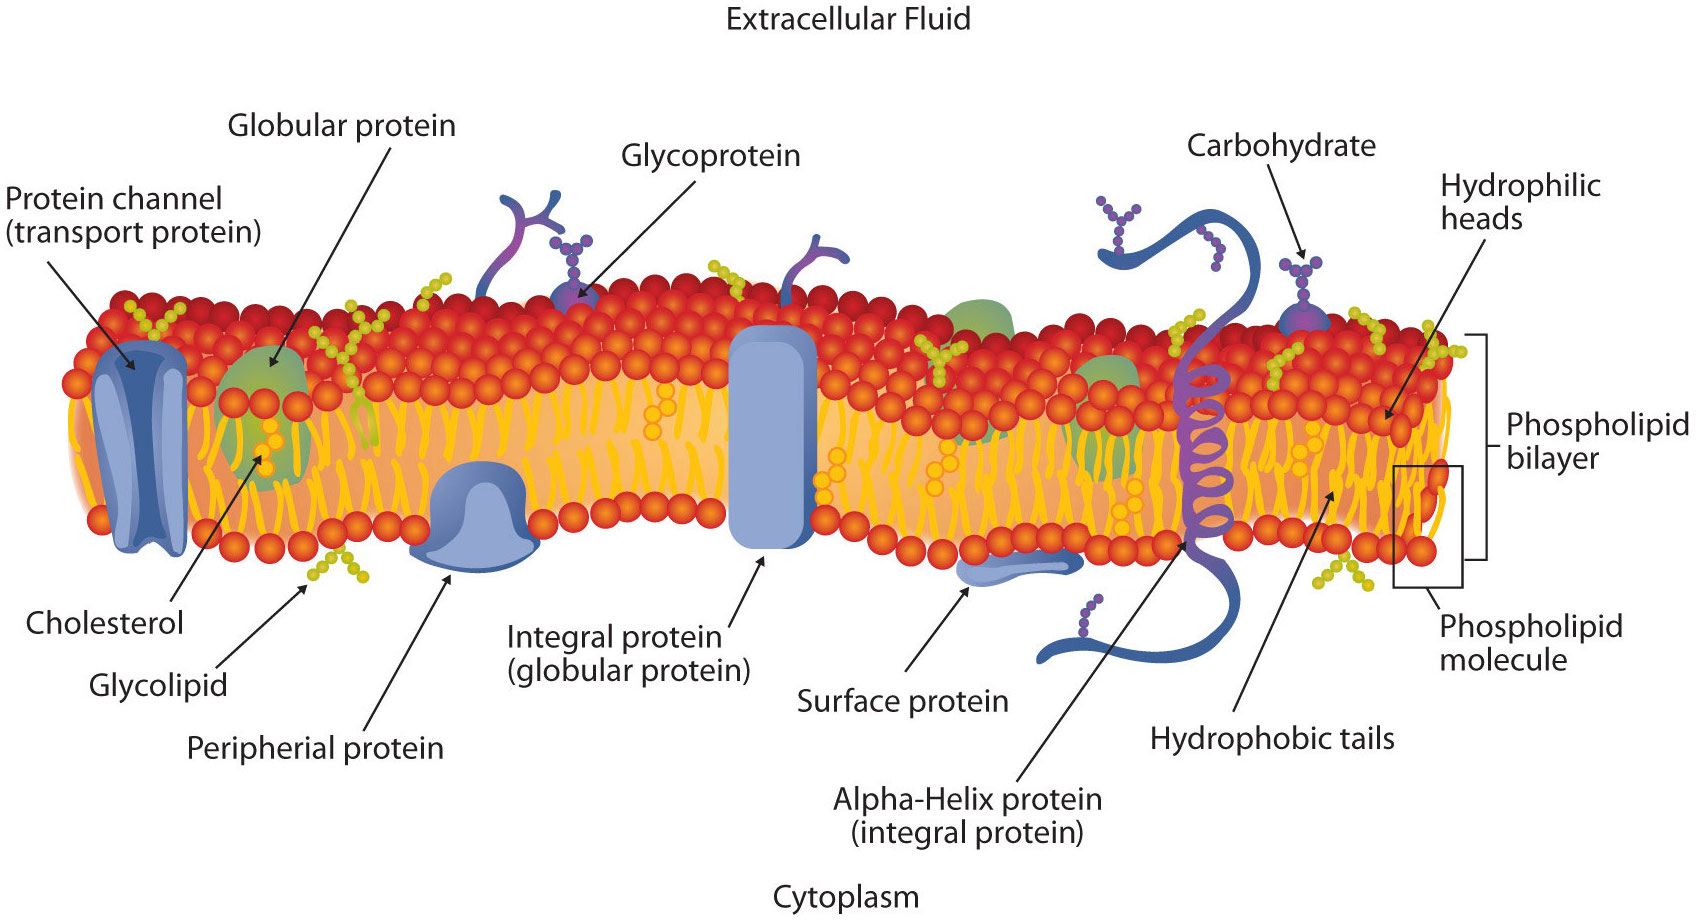
\includegraphics[width=0.9\textwidth]{./img/cellMembrane}
	\caption{Schematic representation of a biological cell membrane.}
	\label{fig:cellMembrane}
\end{figure}

The plasma membrane by mass is essentially composed by half lipids and half proteins. The lipids that constitute the membrane are a particular type of lipids, called \textit{phospholipids}. They are made of a neutral (polar) or charged head, which is hydrophilic and one or two fatty acid hydrocarbon chains, often called lipid tails, which are instead hydrophobic, as shown schematically to the left of figure~(\ref{fig:phospho}). Due to have both properties a phospholipid is an \textit{amphiphilic} molecule. This amphiphilic nature, through the \textit{hydrophobic effect}, play a key role in the membrane formation. In fact when we put a relevant concentration of phospholipids in a water solution at a certain temperature, the lipid tails tend to move away from water molecules due to the hydrophobic effect, so they tend to get closer between them in order to minimize the hydrophobic surface in contact with water. Instead, the polar heads tend to make favorable bonds with water molecules. The resultant bilayer configuration, proper of the biological membrane, is shown schematically to the right of figure~(\ref{fig:phospho}). 
\begin{figure}[!ht]
	\centering
	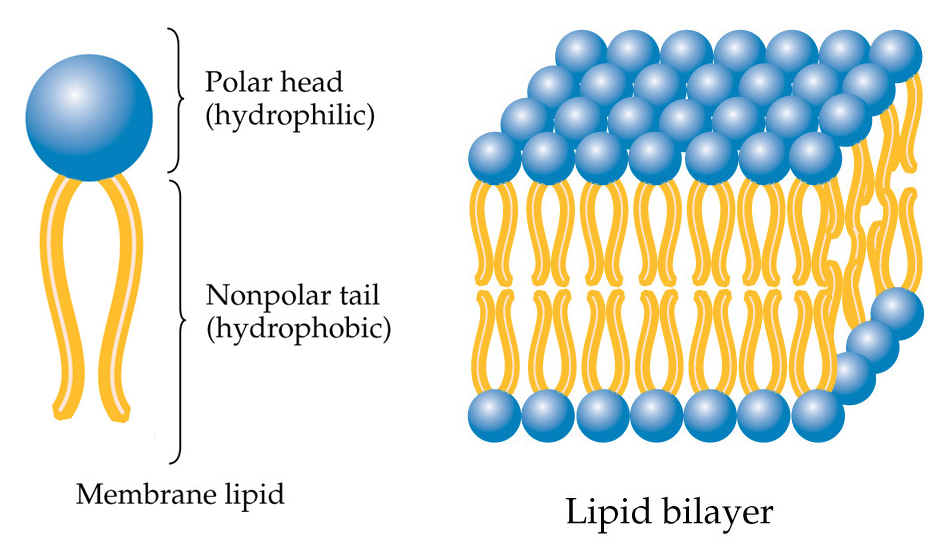
\includegraphics[width=0.6\textwidth]{./img/phospholipids}
	\caption{Left: schematic representation of a phospholipid. Right: self--assembled bilayer configuration assumed by an aqueous solution of phospholipids.}
	\label{fig:phospho}
\end{figure}
Hence, the phospholipids in a water solution tend to \textit{spontaneously} self--organize in a \textit{ordered} state that minimize the Gibbs free energy and that depends on the lipids concentration and the temperature of the solution. As schematically shown in figure~(\ref{fig:lipidsStructures}) the final configurations of such self--assembly process are essentially three: the bilayer sheet, a liposome and a micelle.
\begin{SCfigure}[][!ht]
	\centering
	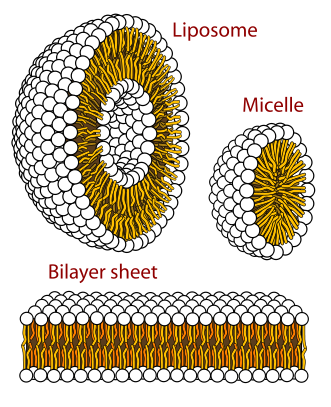
\includegraphics[width=0.35\textwidth]{./img/lipidsStructures}
	\caption{Cross--sectional view of the structures that can be formed by a self--assembly process of a phospholipid aqueous solution.}
	\label{fig:lipidsStructures}
\end{SCfigure}

A real lipid bilayer often contains hundred of different lipid species. They differ in the length of the 
hydrocarbon chains, in the degree of unsaturation, i.e. in the number of double bond in the hydrocarbon chains, 
and in different composition of the head that can be neutral (polar) or charged. There are two main classes of 
phospholipids that make a cell membrane of animals: glycerophospholipid (phosphatidyl--choline, 
phophatidyl--ethanolamine, phophatidyl--serine, phosphatidyl--serine ) and phosphosphingolipids (sphingomyelin). 
In the former group the lipid tails are bound to a glycerol group while the latter do not have glycerol and the 
lipid tails have a backbone of sphingoid bases, absent in the former. These five types take into account for more 
then half of the lipids in most membranes.

The cell membrane has quasi--liquid properties at physiological temperature. This is in part due to some disorder 
in the alignment of the lipid tails produced by the presence of unsaturated chains. Another contribution arise 
from the area occupied by the lipid heads which determines the distance between the hydrocarbon chains. This 
fluid character makes the lipid bilayer like a solvent in which the other molecules (lipids and proteins) are 
dissolved and are free to diffuse. Moreover the lipids itself can move in different ways. The main movements and 
the associated time scales are summarized as follow
\begin{itemize}
	\item lipids conformational change (few nanoseconds);
	\item lipids protrusions out--of--plane (tens of picoseconds);
	\item diffusion within a leaflet (order of tens of nanoseconds);
	\item bilayer undulation and thickness involve collective motion of many lipids.
\end{itemize}
There are also many rare events that take place on the order of hours or even days, such as lipid flip--flop, in 
which a lipid flips from one leaflet to the opposite one; ion translocation; \textit{electroporation} by water, 
for example due to a cross membrane ion imbalance, in which water translocates across the bilayer; water assisted 
ion permeation via formation of a \textit{water--finger} and so forth.

For what concerns the length scales, the bilayer thickness is determined by the length of the lipid tails and 
their degree of unsaturation. Typically the hydrophobic region is $\sim 3$~nm thick while each hydrophilic 
regions is $\sim 1$~nm thick. Hence the typical bilayer thickness is around $\sim 4\div 5$~nm.

\subsection{Model cell membrane}
As we have seen above, the cell membrane is an extremely complex environment due to the large number of different biological molecules (lipids, proteins and so on) which composes and resides in the membrane. The model membranes we will consider in this thesis will be composed of lipids only. This choice is dictated by three main reasons. First, current models and computational power could badly aim at reproducing the complexity of a real plasma membrane. Second, the use of a model system allows to tackle fundamental questions concerning the physical and molecular  ?? interaction between \acp{NP} and membranes, last but not least, the model membrane we will consider resembles closely the model membranes used in a number of experimental and simulations results.  

In the bilayer model we will use, we consider model biological membrane consisting of \ac{POPC} lipids; the 
chemical structure is shown in the top of figure~(\ref{fig:popc}). It is a zwitterionic glycerophospholipid of 
type phosphatidyl--choline whose head is made of a phosphate (PO$_4^-$) and a choline (C$_5$H$_{14}$NO$^+$) 
groups. It has two hydrocarbon chains: one is a saturated chain (palmitoyl) and the other is an unsaturated chain 
(oleoyl). The head groups and tails are both bounded to the glycerol group (C$_3$H$_8$O$_3$).
\begin{figure}[!ht]
	\centering
	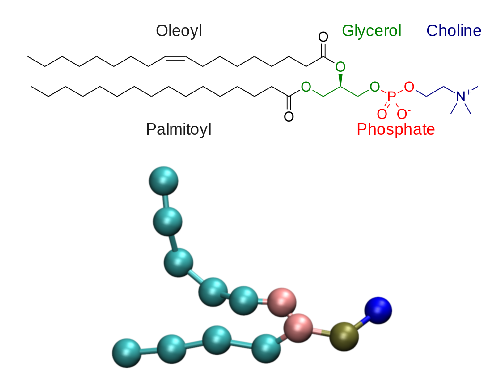
\includegraphics[width=0.7\textwidth]{./img/POPC/popc}
	\caption{Top: chemical structure of a \acs{POPC} lipid. Bottom: \martini \acs{CG} model. The tan bead is the phosphate group, choline is in blue, the two pink beads represents the glycerol group and the hydrophobic chains in cyan.}
	\label{fig:popc}
\end{figure}

\paragraph{\textbf{CG model}} It is clear that the number of lipids that constitute a real cell membrane is 
enormous and it is impossible to take into account an entire cell membrane in a \ac{MD} simulation. A first 
approximation is to consider only a small area of the model bilayer. Given the medium area per lipid of about 
$0.65$~nm$^2$ and a portion of bilayer of $\sim 160$~nm$^2$, which corresponds to about $250$ lipids per leaflet, 
the total number of particles to be included in a atomistic simulation (excluding hydrogen atoms) are about 
$26\cdot 10^3$ plus the water molecules ($\sim 7\cdot 10^4$). This has a very expensive computational cost and 
the range of phenomena which can be studied on these time and length scales are very limited, calling for the 
adoption of a \ac{CG} approach.

\paragraph{\textbf{martini model}} As described in section \ref{sec:martini}, we will use the 
\ac{CG} \martini \ac{FF} for lipids \cite{Martini}.
%We consider a lipid bilayer made of $512$ \ac{POPC} lipids which extend on a surface of about $160$~nm$^2$ and whose thickness is about $4$~nm. 
The \martini model for the \ac{POPC} lipid maps the choline and the phosphate groups into two beads of type Q$_0$ 
and Qa negatively and positively charged, respectively. The saturated tail is modeled with four beads of type 
C$_1$ while the unsaturated tail is built up of four C$_1$ beads and one C$3$ bead which corresponds to the 
unsaturated group of atoms. The glycerol group is modeled with two beads of type N$_\text{a}$. A comparison 
between the chemical structure and \ac{CG} model is shown in figure~(\ref{fig:popc}).

\paragraph{\textbf{model accuracy}} The standard \martini \ac{FF} is able to capture the main physical properties 
of a lipid bilayer. These properties include the area per lipid, the distribution of groups across the membrane, 
the trend of the bending and the area compression moduli in function of the lipids composition and the 
unsaturation degree of the lipids, the stress profile across the membrane, the process of lipid desorption and 
flip--flopping, and many other as better described in \cite{Martini} and \cite{MartiniReview}. Nevertheless many 
other properties, prevalently mediated by the electrostatic interaction, are not well described. As we have seen 
in chapter~\ref{chap:EmpiricalFF}, this is because the \martini \ac{FF} does not take into account the long range 
treatment of the electrostatic interaction and because the standard \martini water is prevalently insensible to 
the electrostatic interaction\footnote{Moreover we can not forget that the \martini water bead takes into account 
four real water molecules. Hence the probability for a \martini water bead to permeate the hydrophobic region of 
the membrane is much less then for a water molecule in an atomistic \ac{FF}.}. To overcome to this problem the 
use of the \ac{PW} model and the \ac{PME} method, as outlined in \cite{MartiniReview} and \cite{PW}, are crucial 
to better describe the process that involve lipid bilayer, water and charged ions. These are ions translocation; 
electroporation of the membrane by water, due to a cross membrane ions imbalance; water--helped ions permeation 
and many other water defects inside the membrane as better described in the works of Marrink and Yesylevskyy. 
Some of the main properties of a pure \ac{POPC} bilayer are shown in table~(\ref{tab:POPCData}) in a comparison 
with different models
\begin{table}[h!t]
	\centering
	\begin{tabular}{lcccc}
		\toprule
		\,				& STD$^a$	& \acs{PME}$^b$	& \acs{PME} + \acs{PW}$^b$ & atomistic$^c$ 	 \\ \toprule
		$D$	[$10^{-8}$~cm$^2$/s]	& $\sim62$	& $44 \pm 4$	& $32.4 \pm 0.7$ & $7.8 \pm 0.9$ \\ \midrule
		$D_{tl}$ [$10^{-8}$~cm$^2$/s] & -		& $36.9 \pm 0.4$& $35 \pm 1$	 & $6.8 \pm 0.2$ \\ \midrule
		$D_{bl}$ [$10^{-8}$~cm$^2$/s] & -		& $45 \pm 3$	& $30.0 \pm 0.6$ & $9.3 \pm 0.1$ \\ \midrule
		$A$ [nm$^2$]				& $0.65$	& $0.630$		& $0.635$		 & $0.688$		 \\ \midrule
		$d$ [nm]					& $4.16$	& $4.29$		& $4.26$ 		 & $3.66$		 \\ \bottomrule
	\end{tabular}
	\caption{Summary of main properties of a pure \acs{POPC} bilayer in comparison with different models. $D$ is the lateral diffusion coefficient of a lipid: in the whole bilayer ($D$), in top leaflet ($D_{tl}$) and in the bottom leaflet ($D_{bl}$). $A$ is the average area per lipid. $d$ is the bilayer thickness as the average distance of the sulphate group. \footnotesize $^a$ Data obtained from \cite{Rossi2014}. $^b$ Data obtained from my \ac{MD} runs. $^c$ Data obtained from \ac{MD} runs by Federica Simonelli.}
	\label{tab:POPCData}
\end{table}

\newpage
\section{NP--Membrane interaction}
Recently the literature concerning the computational modeling about the interaction of anionic 
monolayer--protected \ac{AuNP} and model lipid membranes has expanded contributing to sketch a possible mechanism 
of such interaction. The first step of the interaction between the \ac{NP}, dissolved in the extracellular 
water environment, and the membrane is the attraction between the charged ligands and the polar head of the 
zwitterionic phospholipids: electrostatics it is recognized to be the driving force for the adhesion of the 
\ac{AuNP} to the membrane surface, figure~(\ref{fig:threeProcess}a). To the other end of the pathway, it is 
known, on thermodynamic basis, that the most stable state for the \ac{AuNP} corresponds to the so--called 
\textit{snorkeling} configuration in which the \ac{NP} is embedded in the hydrophobic region of the membrane, 
while the charged ligands stably interact with the lipid heads of both leaflets, 
figure~(\ref{fig:threeProcess}f). 

In the work of Federica Simonelli \etal\, \cite{ourPaper}, using the standard \martini \ac{FF}, the authors found 
and characterized a possible mechanism of the interaction process, as better detailed in the next paragraph. In 
the next paragraph we summarized the findings of Simonelli \etal\,, which constitute the starting point of the 
development of my thesis work.

\subsection{Three--stage process}
%\paragraph{\textbf{Three--stage process}} 
The authors found a three--stage mechanism that regulates the insertion of the \ac{AuNP} into a low curvature 
membrane core: from the adsorbed state, figure~(\ref{fig:threeProcess}a), to the snorkeling configuration, 
figure~(\ref{fig:threeProcess}f). When the \ac{NP} in the water phase is approaching the surface of the membrane 
it enters in the stage $1$, the adsorbed state, in which the charged ligands interact with the polar lipid heads. 
The stage $2$ is the hydrophobic contact, figure~(\ref{fig:threeProcess}d), in which the hydrophobic beads of the 
\ac{MUS} and \ac{OT} ligands are in contact with the hydrophobic tails of the membrane while the charged bead of 
the \ac{MUS} ligands are still in the water phase or in contact with the lipid heads. The stage $3$, is the 
snorkeling configuration, figure~(\ref{fig:threeProcess}f). 

A key role for the stage $1$ to stage $2$ transition is played by a lipid tail protrusion out of the hydrophobic 
region that stably interact with the hydrophobic beads of the \ac{NP} ligands, 
figure~(\ref{fig:threeProcess}b-c). In order to minimize the contacts between water and the tails of the 
protruding lipid it pull the \ac{OT} ligands into the membrane core and the \ac{NP} enter in the hydrophobic 
state, figure~(\ref{fig:threeProcess}d). The lipid tail protrusion mechanism is validate form the 
kinematic of the simulations: the energy barrier to be overcome to move from stage $1$ to stage $2$ is of the 
order of the estimated energy cost of a lipid tail protrusion \cite{VanLehn2015}. Subsequently due to the thermal 
fluctuation a charged bead could cross the membrane core and stably interact with the head region of the opposite 
leaflet bringing the \ac{NP} in the anchored state, figure~(\ref{fig:threeProcess}e).
\begin{figure}[t]
	\centering
	\subfloat[]{
		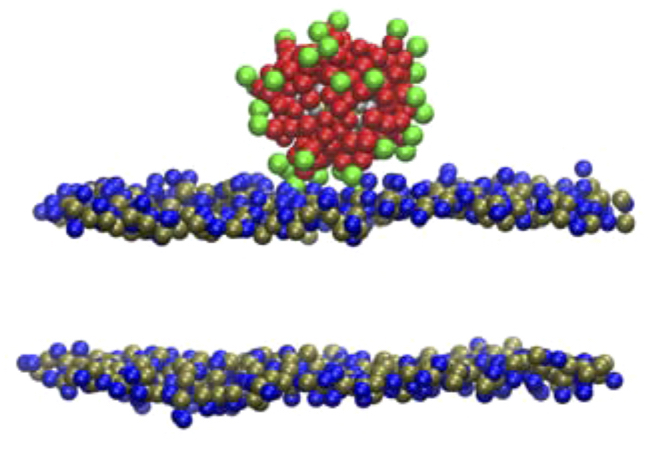
\includegraphics[width=4cm]{./img/threeProcess/a}
	}%
	\quad%
	\subfloat[]{
		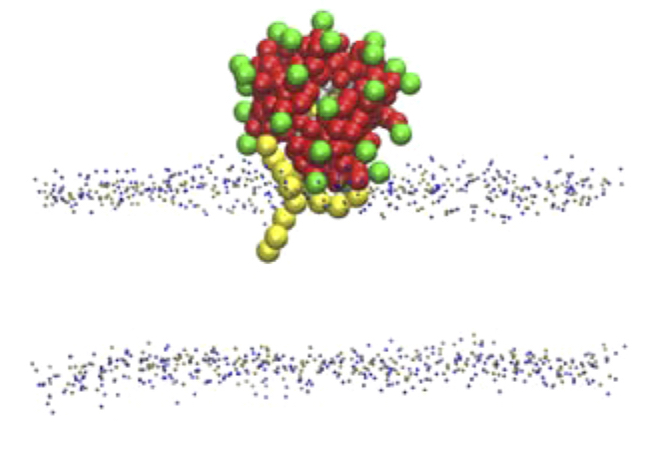
\includegraphics[width=4cm]{./img/threeProcess/b}
	}%
	\quad%
	\subfloat[]{
		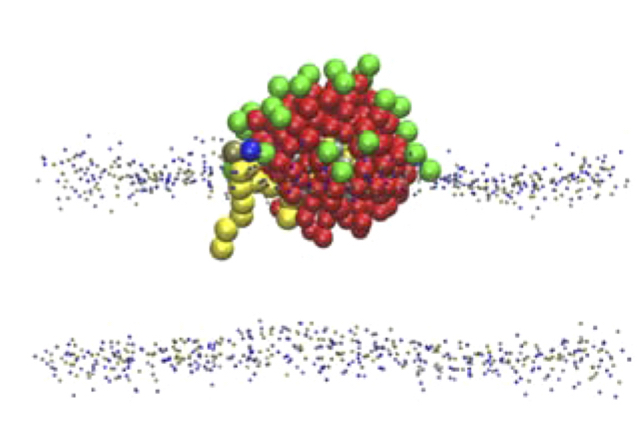
\includegraphics[width=4cm]{./img/threeProcess/c}
	}%
	\\%
	\subfloat[]{
		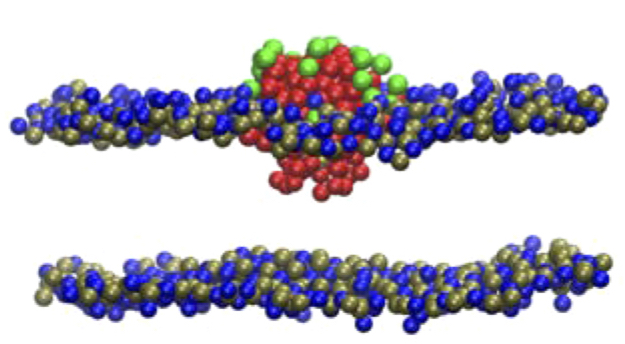
\includegraphics[width=4cm]{./img/threeProcess/d}
	}
	\subfloat[]{
		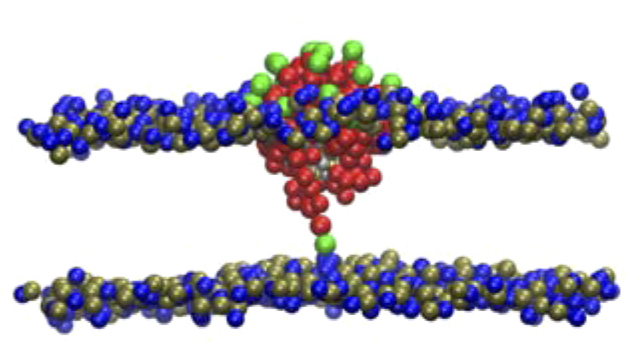
\includegraphics[width=4cm]{./img/threeProcess/e}
	}%
	\quad%
	\subfloat[]{
		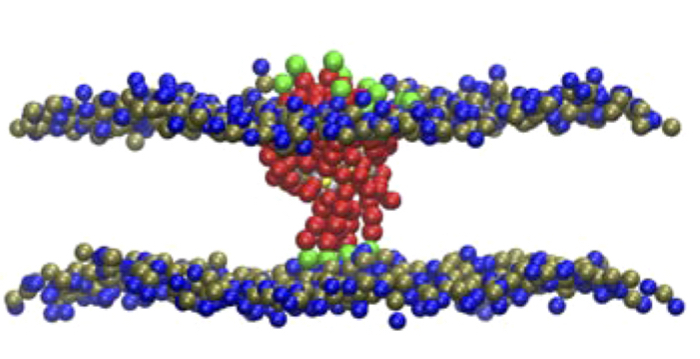
\includegraphics[width=4cm]{./img/threeProcess/f}
	}%
	\caption{\acs{AuNP}--membrane interaction. (a) stage $1$, adsorption of the \acs{NP} at membrane surface; (b) to (d) stage $2$, the protrusion of a lipid tail initiates the hydrophobic contact that leads to partial embedding of the \acs{NP} in the membrane core; (e) the \ac{NP} binds to the opposite leaflet throwing a charged ligand; (f), stage $3$, snorkeling configuration (five anchors shown). The hydrophobic beads of the ligands are shown in red and the charged beads in green. Lipid heads are blue (choline) and tan (phosphate), lipid tails are not shown, expect for (b) and (c), where the protruding lipid is shown with yellow tails. Water beads are not shown. All snapshot refer to a random (\ac{MUS}:\ac{OT} $1$:$1$) configuration. Taken from \cite{ourPaper}.}
	\label{fig:threeProcess}
\end{figure}
Since the anchored state is thermodynamically favorable respect to the hydrophobic state, more and more ligands 
drop the charged beads to the head region of the opposite leaflet, approaching step--by--step the snorkeling 
configuration, figure~(\ref{fig:threeProcess}f). We want to stress out that all the aforementioned transitions 
are triggered by rare molecular event: the lipid tail protrusion and the membrane translocation of a charged 
bead. Hence they could only be observed by the use of a \ac{CG} \ac{FF}. Moreover, compatibly with the other 
works in literature, they found that the energy cost associated with the extraction of the \ac{NP} out of the 
membrane core is very high, making the anchoring process, and the snorkeling configuration, almost irreversible.
 
The authors performed \ac{MD} simulations for the three different \ac{NP} configurations showed in 
figure~(\ref{fig:coating}): the striped (\ac{MUS}:\ac{OT} $1$:$1$), the random (\ac{MUS}:\ac{OT} $1$:$1$) and the 
random (\ac{MUS}:\ac{OT} $2$:$1$). They found that the described behavior is common to the three configurations.  
Nevertheless, after the hydrophobic contact is reached, its lifetime depends on the surface ligand arrangements. 
For the random configurations the time lag between the hydrophobic contact and the first anchor is on the order 
of few nanoseconds. Instead, the striped configuration can linger in the stage $2$ for several microseconds. This 
suggest that the energy barrier to be overcome to move from stage $2$ to the anchored state is less for the 
former than that for the latter. 

\subsection{Preliminary metadynamics results}
\label{sec:preliminaryMetadyn}
To quantify the thermodynamic behavior, Simonelli \etal\, performed metadynamics calculations. In particular, in 
order to estimate the energy barrier for the anchoring process, metadynamics was used to enhance the sampling of 
the transition of the first anchoring ligand from the entrance leaflet to the opposite one. The metadynamics bias 
was apply to the $z$ component of the distance between the center of charged bead and the \ac{COM} of the 
\ac{POPC} bilayer. Then, starting from the hydrophobic state the metadynamics simulations begin biasing the 
charged bead. The convergence of such a run is achieved when the charged bead is able to freely diffuse across 
the membrane. As the size and the complexity of the system does not allow to achieve the convergence, not even at 
\ac{CG} level, the authors decided to perform different statistically independent metadynamics runs and stop each 
\begin{figure}[!b]
	\centering
	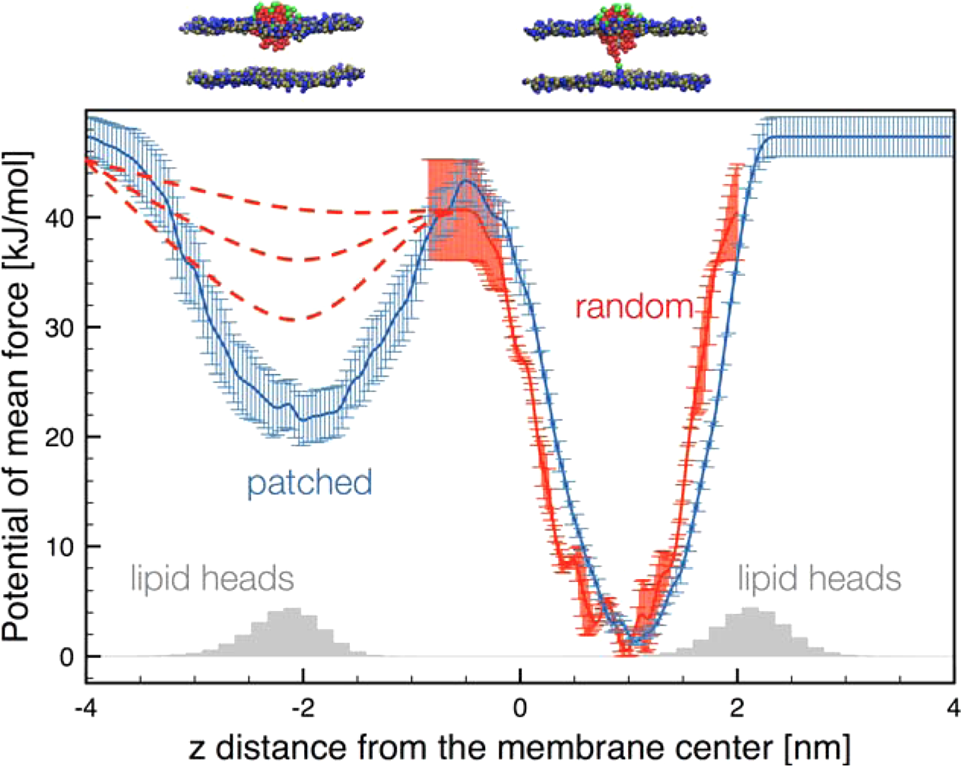
\includegraphics[width=0.6\textwidth]{./img/NPFES}
	\caption{Free energy profile related to the transfer of a negatively charged ligand from the entrance leaflet to the opposite one. The blue is related to the striped (\ac{MUS}:\ac{OT} $1$:$1$) configuration while the red to the random (\ac{MUS}:\ac{OT} $1$:$1$) configuration. Metadynamics data are shown with errorbars, while the red dashed line are hypothesized profiles for the stage $2$ to stage $3$ transition of random \acp{NP}. Gray shades show the position of the polar head beads (AU). Taken from \cite{ourPaper}.}
	\label{fig:NPFES}
\end{figure}
simulation at the recrossing process of the biased ligand. A recrossing is determined when the charged bead is 
$0.5$~nm above the \ac{COM} of the membrane in the leaflet of entrance. The resulting \ac{FES} profile, shown in 
figure~(\ref{fig:NPFES}), is obtained averaging the statistically independent runs. The errorbars are the 
standard error of the independent runs, as described in \ref{sec:metadynamics}.

For the striped arrangement, the crossing barrier to reach the saddle point, located at $0.5$~nm off the \ac{COM} 
of \ac{POPC}, is of the order of $\sim 22$~kJ/mol. While the recrossing energy barrier is approximately twice as 
high. The same is for the recrossing barrier of the random configuration. The absence of data for the random 
\acp{NP} in the hydrophobic contact is due to the difficulty to sample the stage $2$, whose lifetime is too short 
(few nanoseconds).

%to the anchor state transition for only one charged ligand. This is because, while the metadynamics is running on a specific charged ligand, other charged ligands spontaneously anchor to the opposite leaflet, making the free energy sampling of the first anchor impossible. Hence, together with the kinematic, for which the average lifetime of stage $2$ for random \acp{NP} is three order of magnitude shorter than for striped, the authors confirm the very low energy barrier, of the order of few $k_B T$, for the anchor process of the random \acp{NP}.
